
%% bare_conf_compsoc.tex
%% V1.4b
%% 2015/08/26
%% by Michael Shell
%% See:
%% http://www.michaelshell.org/
%% for current contact information.
%%
%% This is a skeleton file demonstrating the use of IEEEtran.cls
%% (requires IEEEtran.cls version 1.8b or later) with an IEEE Computer
%% Society conference paper.
%%
%% Support sites:
%% http://www.michaelshell.org/tex/ieeetran/
%% http://www.ctan.org/pkg/ieeetran
%% and
%% http://www.ieee.org/

%%*************************************************************************
%% Legal Notice:
%% This code is offered as-is without any warranty either expressed or
%% implied; without even the implied warranty of MERCHANTABILITY or
%% FITNESS FOR A PARTICULAR PURPOSE! 
%% User assumes all risk.
%% In no event shall the IEEE or any contributor to this code be liable for
%% any damages or losses, including, but not limited to, incidental,
%% consequential, or any other damages, resulting from the use or misuse
%% of any information contained here.
%%
%% All comments are the opinions of their respective authors and are not
%% necessarily endorsed by the IEEE.
%%
%% This work is distributed under the LaTeX Project Public License (LPPL)
%% ( http://www.latex-project.org/ ) version 1.3, and may be freely used,
%% distributed and modified. A copy of the LPPL, version 1.3, is included
%% in the base LaTeX documentation of all distributions of LaTeX released
%% 2003/12/01 or later.
%% Retain all contribution notices and credits.
%% ** Modified files should be clearly indicated as such, including  **
%% ** renaming them and changing author support contact information. **
%%*************************************************************************


% *** Authors should verify (and, if needed, correct) their LaTeX system  ***
% *** with the testflow diagnostic prior to trusting their LaTeX platform ***
% *** with production work. The IEEE's font choices and paper sizes can   ***
% *** trigger bugs that do not appear when using other class files.       ***                          ***
% The testflow support page is at:
% http://www.michaelshell.org/tex/testflow/



\documentclass[conference,compsoc]{IEEEtran}
% Some/most Computer Society conferences require the compsoc mode option,
% but others may want the standard conference format.
%
% If IEEEtran.cls has not been installed into the LaTeX system files,
% manually specify the path to it like:
% \documentclass[conference,compsoc]{../sty/IEEEtran}

\usepackage[T5]{fontenc}
\usepackage[utf8]{inputenc}

\usepackage{xcolor}
\usepackage{pgfplots}
\usepackage{tikz}

% Define bar chart colors
%
\definecolor{bblue}{HTML}{4F81BD}
\definecolor{rred}{HTML}{C0504D}
\definecolor{ggreen}{HTML}{9BBB59}
\definecolor{ppurple}{HTML}{9F4C7C}


% Some very useful LaTeX packages include:
% (uncomment the ones you want to load)


% *** MISC UTILITY PACKAGES ***
%
%\usepackage{ifpdf}
% Heiko Oberdiek's ifpdf.sty is very useful if you need conditional
% compilation based on whether the output is pdf or dvi.
% usage:
% \ifpdf
%   % pdf code
% \else
%   % dvi code
% \fi
% The latest version of ifpdf.sty can be obtained from:
% http://www.ctan.org/pkg/ifpdf
% Also, note that IEEEtran.cls V1.7 and later provides a builtin
% \ifCLASSINFOpdf conditional that works the same way.
% When switching from latex to pdflatex and vice-versa, the compiler may
% have to be run twice to clear warning/error messages.






% *** CITATION PACKAGES ***
%
\ifCLASSOPTIONcompsoc
  % IEEE Computer Society needs nocompress option
  % requires cite.sty v4.0 or later (November 2003)
  \usepackage[nocompress]{cite}
\else
  % normal IEEE
  \usepackage{cite}
\fi
\hyphenation{op-tical net-works semi-conduc-tor}


\begin{document}
%
% paper title
%\title{OMNN at VLSP-2016 OM\\}
\title{A Multi-layer Neural Network-based System for Vietnamese Sentiment Analysis at the VLSP 2016 Evaluation Campaign\\}


\author{\IEEEauthorblockN{Thy Thy Tran\IEEEauthorrefmark{1},
Xanh Ho\IEEEauthorrefmark{2} and Nhung T.H. Nguyen\IEEEauthorrefmark{3}}
\IEEEauthorblockA{Faculty of Information and Technology\\   
VNUHCM University of Science\\
Email: \IEEEauthorrefmark{1}thy2512@gmail.com,
\IEEEauthorrefmark{2}xanhhocntt@gmail.com,
\IEEEauthorrefmark{3}nthnhung@fit.hcmus.edu.vn}}



% make the title area
\maketitle

% As a general rule, do not put math, special symbols or citations
% in the abstract
\begin{abstract}
We present a description of our system submitted to the VLSP 2016 Evaluation Campaign of Sentiment Analysis for the Vietnamese Language. This year the campaign focussed on polarity classification, i.e., to classify Vietnamese reviews or documents into positive, negative or neutral. In order to address the task, we implemented a multi-layer neural network-based method that uses three types of features as input. Our internal evaluations indicate that by using TF-IDF feature to represent sentences, we can obtain the best performance with 66\% of precision and 65\% of recall. The official accuracy of the proposed method on the testing set (evaluated by the organiser) is 65.9\%.
\end{abstract}

% no keywords

\IEEEpeerreviewmaketitle

\section{Introduction}
Recently, with the explosive of social media, there is a high demand from brands and industries to automatically analyse the customers’ comments on their products so that they can know how consumers perceive their products as well as those of their competitors. This sentiment information is not only useful for marketing and product benchmarking but also useful for product design and product development~\cite{liu2012sentiment}. 
Extracting opinion or sentiment from text can be defined as sentiment analysis or opinion mining. The task receives raw texts talking about brands or products as input, and outputs sentiment information, which indicates the author’s opinions about a specific brand, product, or about products’ features. In general, the task of sentiment analysis can be divided into three levels: document-based, sentence-based, and aspect-based. The VLSP 2016 evaluation campaign of sentiment analysis for the Vietnamese language focussed on the first level\footnote{\url{http://vlsp.org.vn/evaluation\_campaign\_OM}}, i.e., classify input documents or reviews into one over three sentiment classes: positive, negative and neutral.

Most approaches for sentence-based sentiment analysis are supervised learning-based methods such as Naive Bayes, support vector machine (SVM) and neural networks (NN). In this paper, we have implemented multilayer NN (MLNN) for Vietnamese sentiment analysis. Specifically, our model is a fully connected neural network with only one hidden layer and gets feature vector as input. We have conducted experiments to compare the proposed method with SVM implementation from scikit-learn~\cite{scikit-learn} and fastText from facebook~\cite{joulin2016bag}. For SVM, we also extract the same features that we use for MLNN. Meanwhile, regarding fastText, the model first randomizes a weight matrix that is a lookup table over words, then the word representations are averaged into a text representation and experience classification on it. Experimental results show that MLNN with TF-IDF feature as input produced the best scores among the models. We have applied the best performing method to the testing set and obtained an official accuracy of 65.9\%.

%While research in this field for English has obtained state-of-the-art status~\cite{}, there is a few work for Vietnamese~\cite{Kieu_2010,Ha_2011,Hong_2014,Duyen_2014}. Furthermore, there is no available gold standard to systematically evaluate performances of Vietnamese sentiment analysis systems. In order to alleviate such issues

\section{Related Work}
\label{related}
%Sentiment analysis has been being studied since the 2000s. So far, 
%The appearance from the 2000s, up-to-date sentiment analysis got many successes on this field.
%Similar to other NLP problems, approaches for document-based sentiment analysis can be divided into unsupervised and supervised learning~\cite{liu2012sentiment}.
%Sentiment classification using supervised learning is usually divided into two classes: positive and negative.
%Navie Bayes and support vector machine (SVM)~\cite{cristianini2000, Joachims98makinglarge_scale} with feature bag of words (Pang et al. 2002~\cite{Pang02thumbsup}) as are first technique been used to sentiment classification.
%Then, many studies effective features, such as text topic~\cite{Ganu_beyondthe}, sentiment words, and phrases~\cite{Tong2001} 
%and sentiment lexicon features~\cite{sentiment_kiritchenko}.
%Recently, neural networks have been applied to many natural language processing problems and sh to be promising and effective emerged and achieved promising results for sentiment classification. 
%Approaches of neural networks can divide two methods: learning word embeddings and learning semantic composition. 
%(Mikolov et al., 2013~\cite{mikolov:distributed}; Pennington et al., 2014~\cite{pennington2014glove}) used local and global contexts in learning word embeddings. Meanwhile, for learning semantic composition, Socher et al. (2013)~\cite{Socher-etal:2013} introduce a family of recursive deep neural networks (RNN).

While research on sentiment analysis for English has been being grown and obtained the state of the art~\cite{Tong2001,Pang02thumbsup,sentiment_kiritchenko,Ganu_beyondthe,SocherEtAl2011:RAE}, there is a few work for Vietnamese. 
Kieu and Pham~\cite{Kieu_2010} introduced a rule-based system using the GATE framework for sentence-level sentiment analysis. They conducted their experiments on a corpus of computer product reviews and obtained 61.16\% of precision, 64.62\% of recall.
Ha et al.~\cite{Ha_2011} described an extension of a feature-based opinion mining and summarizing model to extract sentiments from reviews on mobile phone products. 
Feature words and opinion words were extracted based on some Vietnamese syntactic rules. Opinion orientation and summarization on features were determined by using VietSenti WordNet.
Their model produced 69.16\% of precision and 68.86\% of recall.
Nguyen et al.~\cite{Hong_2014} proposed an approach extract opinions from Vietnamese documents using a domain specific sentiment dictionary. 
The sentiment dictionary is built incrementally by applying statistical methods to 20,083 comments about mobile products crawled from the Internet. 
Nguyen et al.~\cite{Duyen_2014} introduced an annotated corpus for document-level sentiment analysis that consists of hotel reviews. They implemented several machine learning-based methods that use different types of features. Their experimental results indicated that using word-based features produced better performance than using syllable-based ones. Among different types of $n$-grams, only unigrams were effective for the task.

%presented an empirical study on machine learning, introduce an annotated corpus for sentiment classification extracted from hotel reviews, and showed information about sentiment classification in Vietnamese such as using word-based features achieved the better results than using syllable-based, using only unigrams was effective for the task.


\section{System Overview}
For each input document, we extract a feature vector that can represent as exactly as possible the characteristic of the input. Specifically, we extract three types of features: Bag-Of-Word (BOW), TF-IDF and SentiWordNet-based features.
%We consider the task of sentiment analysis as a classification task, in which we extract features from each sentence and classify the sentence into positive, negative or neutral class. Specifically, we extracted three features of a sentence: Bag-Of-Word (BOW), TF-IDF and SentiWordNet-based features.
Then, each document vector based on the above features along with its label will be fed to a classifier to learn a model that can determine the sentiment class.

\subsection{Feature Extraction}
BOW and TF-IDF are common features that have been used in text mining as well as other NLP problems. While SentiWordNet-based features are extracted based on VietSenti Wordnet~\cite{Xuan-Son-Vu:2014}--a lexicon resource that contains sentiment expressions and its three types of scores. Details about these features will be presented below.
%We present the details of the features have been tried out in this paper but not all of them were included in the final submitted model. 
% In addition to common text mining features such as BOW and TF-IDF, our approach extracts other features based on VietSentiWordnet~\cite{}--a lexicon resource that contains sentiment expressions and its three types of scores. Details about these features will be presented below.
%We give a short explanation of our used features below:
%\paragraph{\textbf{BOW}}
\subsubsection{BOW}
Each review is represented by a sparse vector as the bag of its words over a fixed vocabulary, ignoring grammar and word order.

\subsubsection{TF-IDF}}
TF-IDF reflects how importance is a word to a document in the corpus. It is composed by two terms: (1)Term Frequency (TF) computes the number of times that word occurs in the current document, and (2) Inverse Document Frequency (IDF) shows how much information a term provides. In this work, we use TF-IDF scores as review representation vectors.

\subsubsection{SentiWordnet-based}
VietSentiWordNet\cite{Xuan-Son-Vu:2014} is a synset of words that express sentiment. However, it contains not only sentiment words but also phrases with some included sentiment shifter such as \textit{not}. Therefore, we have to extract $n$-gram, range from unigram to pentagram, to map vocabulary of VietSentiWordnet. In details, we use the lexicon in three ways: \begin{itemize}
    \item \textbf{BOW-senti} We extract the BOW feature based on a fixed vocabulary extracted from VietSenti Wordnet. The whole collocation contains 1198 terms with their corresponding frequency of $n$-grams showed in Table \ref{tb-senti}.
   
    \item \textbf{TF-IDF-senti} We also used the VietSentiWordnet to compute TF-IDF scores.
    \item \textbf{Objectivity-score} The Wordnet also provides information of the sentiment scores involving positive, negative, and objectivity scores extracted from positive and negative as 
    \[ObjScore = 1 - (PosScore + NegScore)\]
    Based on the objectivity score, we build a feature vector represents VietSenti Wordnet, for each sentiment word/phrase appears in a sentence, we add its corresponding objectivity score.
\end{itemize}

 \begin{table}[t]
    \centering
    \caption{VietSentiWordnet $N$-gram occurence}
    \label{tb-senti}
    \begin{tabular}{c|r|c}
    \textbf{$N$-gram} & \textbf{Count} & \textbf{Example} \\
    \hline
    \textbf{1-gram} & 885 & 'khủng\_khiếp' \\
    \textbf{2-gram} & 236 & 'tốt nhất' \\
    \textbf{3-gram} & 61 & 'giá quá cao'  \\
    \textbf{4-gram} & 13 & 'không có ý định' \\
    \textbf{5-gram} & 3 & 'không tạo được cảm\ hứng' \\ 
    \end{tabular}
\end{table}

%\begin{equation}
%    ObjScore = 1 - (PosScore + NegScore)
 %   \label{eq-objscore}
%\end{equation}

% three different feature include tf-idf scores, tf-idf with fixed vocabulary from VietSenti Wordnet, and sentiment scores in VietSenti Wordnet.



% https://en.wikipedia.org/wiki/Tf\%E2\%80\%93idf


% http://trimc-nlp.blogspot.com/2013/04/tfidf-with-google-n-grams-and-pos-tags.html

% https://aclweb.org/anthology/S/S16/S16-1010.pdf

\subsection{Classification}
In this work, we use three different algorithms to classify reviews' polarity. The first one is a linear \textbf{support vector machine} (\textbf{SVM}) classifier provided by the scikit-learn toolkit \cite{scikit-learn}. The second is an implementation of \textbf{multilayer neural network} (\textbf{MLNN}) using NumPy which provides multidimensional arrays and functions \cite{Walt:2011:NAS:1957373.1957466}. The last is an extra experiment using a recent released library named \textbf{fastText}\cite{joulin2016bag}.

Regarding the SVM classifier, we use the linear kernel which handles multiclass classification by a one-vs-rest scheme. In details, the strategy involves training a single classifier per class in order to produce a confidence score for its decision, then the label that has the highest confidence would be the predicted class.

For the MLNN model, we conducted experiments with several architectures and hyperparameters include learning rate, and $l2$ regularization scale. Specifically, we use Stochastic Gradient Descent (SGD) to optimize the objective function and use a flag for early stopping if the validation accuracy is not increased after 20 epochs. The extracted features will be used as input to the network.

For comparison, we also train a supervised classifier using fastText, which is a library for learning word representations and sentence classification introduced by Facebook.

We evaluate all the above-mentioned models using cross-validation to assess how the models generalize for an independent data.

\section{Experiments}
\subsection{Dataset}
The provided data this year (2016) is in the domain of technical devices, of which the training data consists of 5100 reviews with an equal proportion for each sentiment class. The data distribution is presented in Table \ref{tb-stt}. A noticeable point is that a neutral label will be assigned to a review if the review contains both positive and negative opinions. Table \ref{tb-ex} illustrates this phenomenon, which makes the classification task more difficult.

\begin{table}[t]
\centering
\caption{Characteristics of the provided data}
\label{tb-stt}
\begin{tabular}{l|r|r|r|r}
               & \textbf{POS} & \textbf{NEG} & \textbf{NEU} & \textbf{Total} \\
\hline
\textbf{TRAIN} & 1700         & 1700         & 1700         & 5100           \\
\textbf{TEST}  & 350          & 350          & 350          & 1050          
\end{tabular}
\end{table}

\begin{table}[t]
\centering
\caption{A review that is labeled as neutral since it contains both positive and negative sentiment}
\label{tb-ex}
\begin{tabular}{|l|}
\hline
Rất tốt nha bạn , hơi cấn ngón\_cái chút vì có hai nút bấm gồ lên ,\\xài lâu cũng quen , hơi nặng chút , nếu bạn xài Mac nên đầu\_tư \\một con mighty để bàn , con này đem đi\_lại , về kết\_nối bluetooth\\thì cảm\_giác lag hơn Magic\_mouse , còn nếu dùng usb receiver thì\\ rất ngon , battery thì mình dùng một tháng nay chưa hết ,\\không\_bao\_giờ Off nguồn .\\
\hline
\end{tabular}
\end{table}

% data distribution


\subsection{Evaluation Metrics}

% [pos, neg, neu]
Evaluation metrics in this work include accuracy, precision, recall, and F1 score. However, we only compute the last three ones for each model while running cross-validation, including the average scores for three categories (positive, negative, and neutral) and the total scores overall. The purpose is to select the best performing model that will be applied to the official testing set of the sentiment analysis campaign.

\subsection{Experimental Results}

%We divide our evaluation results based on the main model but not feature. At first, 
Table \ref{tb-SVM} presents the performances of SVM when we use five separate features as input through cross-validation. Overall, TF-IDF obtains the highest scores for all precision, recall, and F1 with 0.65, 0.65 and 0.65, respectively. Meanwhile, the performance when using features extracted from the VietSenti Wordnet, is even worse than that of BOW. 
%the  In addition, the use of VietSenti Wordnet even gets lower scores for the sentiment classification task, with the highest F1-score is 0.47 compared to 0.61 and 0.65 for BOW and TF-IDF, respectively.

\begin{table}[t]
\centering
\caption{Performances of SVM with different types of features}
\label{tb-SVM}
\begin{tabular}{|l|c|c|c|}
\hline
\textbf{SVM}             & \textbf{Precision} & \textbf{Recall} & \textbf{F1-score} \\ \hline
\textbf{BOW}             & 0.61               & 0.62            & 0.61              \\
\textbf{TF-IDF}          & \textbf{0.65}      & \textbf{0.65}   & \textbf{0.65}     \\
\textbf{BOW-senti}       & 0.44               & 0.38            & 0.34              \\
\textbf{TF-IDF-senti}    & 0.44               & 0.39            & 0.34              \\
\textbf{Objectivity-score} & 0.49               & 0.48            & 0.47              \\ \hline
\end{tabular}
\end{table}

Regarding MLNN, we designed its architecture as follows. The input layer has a dimension that depends on the dimension of the feature vectors. The hidden layer has 100 computational units. The last layer with 3 neurons stands for the number of labels which is positive, negative, and neutral. The neural structure was chosen as the model that produces the best results after several running and evaluating using cross-validation
%Another feature-based approach used in this work is MLNN.
%In details of our MLNN architecture, it is an input which dimension depends on the feature set, next is hidden layer with 100 computational units, and the last layer with 3 neurons stands for the number of labels which is positive, negative, and neutral. The neural structure was chosen as the model gave the best results after several running and evaluating using cross-validation.
Table \ref{tb-NN} shows the performance of MLNN using the same features with SVM. As can be seen, using TF-IDF as input for MLNN also performs the best among our features, similarly to SVM. Specifically, the F1-score over the three sentiment classes is also 0.65, which is equal to the best score produced by SVM. However, MLNN produces a little higher precision score (0.66 vs. 0.65 by SVM). 
%This is the resTherefore, we choose it as the final model to classify the test data of the campaign.


\begin{table}[t]
\centering
\caption{Performances of MLNN with different types of features}
\label{tb-NN}
\begin{tabular}{|l|c|c|c|}
\hline
\textbf{MLNN}             & \textbf{Precision} & \textbf{Recall} & \textbf{F1-score} \\ \hline
\textbf{BOW}             & 0.64               & 0.63            & 0.63              \\
\textbf{TF-IDF}          & \textbf{0.66}      & \textbf{0.65}   & \textbf{0.65}     \\
\textbf{BOW-senti}       & 0.43               & 0.37            & 0.29              \\
\textbf{TF-IDF-senti}    & 0.39               & 0.37            & 0.30              \\
\textbf{Objectivity-score} & 0.47               & 0.45            & 0.43              \\ \hline
\end{tabular}
\end{table}

Training a classifier using fastText is a bit different with that for SVM and MLNN. We do not need to feed into the input layer the extracted features, the model already contains a random initialization weight matrix as a word representation look up table. The matrix would be adjusted through the training step. Then, the text representation is composed by averaging its word representations before transform to the classification layer.
%In the following, we present the results from a supervised classification model trained using fastText. The model classifies from a review representation vector that comes from averaging its word representations. of precision and Table \ref{tb-fast} shows information of the model performance, it only attains 0.498 of precision on the training data. Therefore, the model could not be considered to perform the classification on the test set.
By using fastText, we obtained the same scores of precision and recall with 0.498. 

%\begin{table}[t]
%\centering
%\caption{Classification using fastText}
%\label{tb-fast}
%\begin{tabular}{l|c|c}
%  & \textbf{Precision} & \textbf{Recall} \\ \hline
%\textbf{fastText} & 0.498              & 0.498          
%\end{tabular}
%\end{table}


Among the three classifiers, when using SVM and MLNN with TF-IDF features, we obtained the best score of 0.65 F1-score. However, precision produced by MLNN is a little bit higher than that by SVM. Therefore, we select MLNN with TF-IDF features to apply to the official testing set of the campaign. The results on the testing set are presented in Table \ref{tb-test}. 


\begin{table}[htp!]
\centering
\caption{Official testing results on individual class. The overal accuracy is 65.9\%}
\label{tb-test}
\begin{tabular}{|c|c|c|c|}
\hline
    \bf Class        & \multicolumn{1}{l|}{\textbf{Precision}} & \multicolumn{1}{l|}{\textbf{Recall}} & \textbf{F1-score} \\ \hline
\textbf{POS} & 69.06                                   & 71.43                                & 70.23             \\ \hline
\textbf{NEG} & 65.67                                   & 62.86                                & 64.23             \\ \hline
\end{tabular}
\end{table}
    
\subsection{Discussion}
The above-mentioned experimental results indicate that with this specific data of Vietnamese sentiment analysis, SVM and MLNN produce comparable scores for all metrics. This situation is a bit conflict with the trend in English natural processing, in which neural networks beat state-of-the-art in many areas such as speech recognition\cite{NIPS2010_0160}, language modeling\cite{mikolov2012statistical}, and especially sentiment classification \cite{SocherEtAl2011:RAE}. 
However, such situation can be explained by the fact that the provided training data is smaller than that for the English. Our dataset involves only 146,440 tokens and the vocabulary size is only 2,248 words. Meanwhile, to obtain the state-of-the-art, the English sentiment tree bank consists of 184,837 tokens with informative treebanks. This means that in order to effectively train a neural network-based model, we need a bigger training data with more linguistic information.

%, but as showed in the experiments section, it performs worser than feature based models. It is probably understandable that we need a huge amount of data for training word or sentence representation while our dataset involves only 146,440 tokens and the vocabulary size is only 2248 words.

Another interesting phenomenon is that, although the training data has a balanced ratio of sentences in each class, the average length among them is quite significant different as showed in Table \ref{tb-len}. The average length of a neutral review is nearly 6 to 7 words longer than a positive or negative review. Likewise, the number of tokens in neutral reviews is also close to twice times of that in positive or negative ones. These points make the problem hard to solve the imbalance word occurrence over three classes. Even in our final model, the average performance through cross-validation also bias to learn well on positive class than the other two, and often classify the neutral label incorrectly (see Figure \ref{fig-mlnn}).

\begin{table}[t]
\centering
\caption{Average length (in words) of documents in the training data}
\label{tb-len}
\begin{tabular}{l|r|r|r|r}
                       & \textbf{POS} & \textbf{NEG} & \textbf{NEU}   & \textbf{Total} \\ \hline
\textbf{Avg. length}   & 11.67        & 12.60        & \textbf{18.79} & 14.36          \\ \hline
\textbf{Num of tokens} & 39689        & 42845        & \textbf{63906} & 146440        
\end{tabular}
\end{table}


\begin{figure}[t]
        \centering
        \caption{Precision, Recall and F1-score of MLNN using TF-IDF over three categories: positive (POS), negative (NEG) and neutral (NEU)}
        \label{fig-mlnn}
        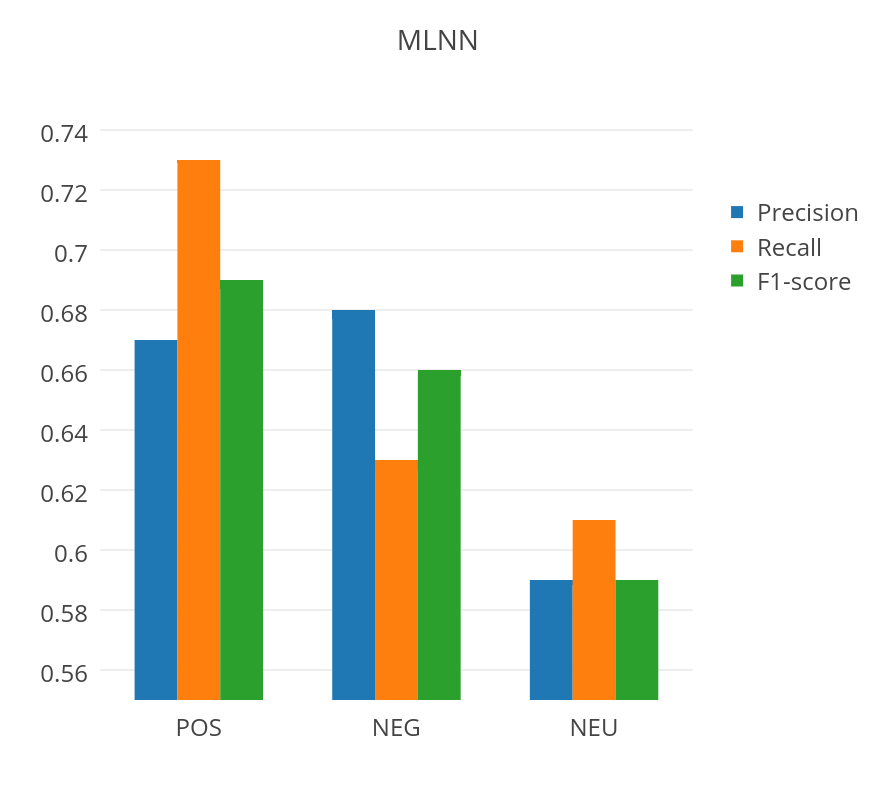
\includegraphics[scale=0.25]{./png/MLNN-vlsp}
\end{figure}


    
\section{Conclusion}
This paper has described our system submitted to the sentiment analysis evaluation campaign of the VLSP 2016. To conclude, for small data, the traditional feature is still better than neural networks with word representation.
Due to the limited collocation of the SentiWordnet, it is not a good choice to use separately as the only feature. Moreover, our experiments only use distinct features as input without combining them, it should be considered as an avenue for the further work.




\bibliographystyle{IEEEtran}
% argument is your BibTeX string definitions and bibliography database(s)
\bibliography{IEEEexample}

% \end{thebibliography}




% that's all folks
\end{document}


